
\documentclass[brazil]{beamer}

\usepackage[utf8]{inputenc}
\usepackage{babel}

\usepackage{pgfpages}

\setbeameroption{show notes on second screen=right}

\usetheme[
    titleformat=allcaps,
    progressbar=foot,
    block=fill]{metropolis}           % Use metropolis theme

\usepackage{tikz}
    \usetikzlibrary{shapes.symbols, shapes.callouts, arrows, calc, backgrounds, fit}
    
    \makeatletter
    \newcommand{\gettikzxy}[3]{%
      \tikz@scan@one@point\pgfutil@firstofone#1\relax
      \edef#2{\the\pgf@x}%
      \edef#3{\the\pgf@y}%
    }
    \makeatother

    \tikzstyle{arrow} = [thick,->,>=stealth]

\usepackage{subfigure}
\usepackage{graphicx}

\usepackage{hyperref}
\usepackage{textcomp}

%% Para estilizar emails
\catcode`\_=11\relax
\newcommand\email[1]{\_email #1\q_nil}
\def\_email#1@#2\q_nil{%
    \textlangle{}\href{mailto:#1@#2}{{\emailfont\detokenize{#1}\emailampersat\detokenize{#2}}}\textrangle{}%
}
\newcommand\emailfont{\ttfamily}
\newcommand\emailampersat{{\color{red}\small@}}
\catcode`\_=8\relax
%% --

\usepackage[autostyle,portuguese=brazilian]{csquotes}

    \def\signed #1{{\leavevmode\unskip\nobreak\hfil\penalty50\hskip1em
    \hbox{}\nobreak\hfill #1%
    \parfillskip=0pt \finalhyphendemerits=0 \endgraf}}

    \newsavebox\mybox
    \newenvironment{aquote}[1]
    {\savebox\mybox{#1}\begin{quote}\openautoquote\hspace*{-.7ex}}
    {\unskip\closeautoquote\vspace*{1mm}\signed{\usebox\mybox}\end{quote}}

\usepackage{transparent}

\title{Estruturas de Dados \\ e Viagem no tempo}
\date{\vspace*{1.5em} \large V SESCOMP --- 2019}
\author{{{\Large Arthur Araruna}\raisebox{1ex}{$\alpha$}} \\ \scriptsize \email{ararunaufc@gmail.com}}
\institute{\vspace*{3em} \scriptsize \raisebox{1ex}{$\alpha$}Universidade Federal do Ceará \\ \hphantom{\raisebox{1ex}{$\alpha$}}Campus de Quixadá}

\begin{document}
    \logo{
\includegraphics[height=.8cm]{../../ufc-qxd-hor-col.png} \hspace*{.3cm}}
    \frame{
        \titlepage
        \note{Apresentação pessoal}
        \note[item]{Experiência acadêmica}
        \note[item]{Experiência docente}
        \note[item]{Interesses acadêmicos}
    }

    \logo{\transparent{0.4}
\includegraphics[height=.8cm]{../../ufc-qxd-hor-col.png} \hspace*{.3cm}}
    \begin{frame}
        \frametitle{Ressalvas}
        
        \begin{itemize}[<+->]
            \item Duas palestras pelo preço de uma.
            \begin{itemize}
                \item Na verdade, um apanhado + uma visão geral
            \end{itemize}
            \item {\em Viagem no tempo}: não-especialista, não-estudioso, apenas um deslumbrado.
            \item {\em Estruturas temporais}: não-especialista, mas entusiasta.
            \begin{itemize}
                \item Dar o pontapé inicial no estudo dessas estruturas
                \item Como desculpa, falar sobre viagem no tempo
            \end{itemize}
        \end{itemize}
    \end{frame}

\section{Viagem no Tempo ---  segundo a física}

    \begin{frame}
    \frametitle{Viagem no tempo}

    \alert{\Large É possível viajar no tempo?}

    \uncover<2->{Resposta curta: {\bfseries sim!}}
    \begin{itemize}
        \item<3-> Para o futuro: \uncover<4->{\em viver}
        \item<3-> Para o passado: \uncover<5->{\em lembrar}
    \end{itemize}
\end{frame}

\begin{frame}
    \frametitle{Viagem no tempo}

    {\Large É possível viajar no tempo \alert{fora do trivial}?}

    \uncover<2->{Resposta curta: {\bfseries talvez...}}
\end{frame}

\subsection{Viagem ao futuro}

\begin{frame}
    \frametitle{Segundo a Física Clássica}

    \begin{block}{Física Newtoniana}
        \begin{itemize}
            \item Tempo é absoluto
            \begin{itemize}
                \item Noção de ``relógio global''.
                \item Passagem do tempo acontece na mesma proporção para todos os lugares do universo.
            \end{itemize}
            \item Tempo é irrefreável
            \begin{itemize}
                \item ``O espaço'' acontece várias e várias vezes, e o que usamos para rotular as ocorrências é ``o tempo''.
                \note[item]{Espaço-tempo como um filme de projetor.}
            \end{itemize}
        \end{itemize}
    \end{block}
    \only<2->{De uma certa forma, a viagem no tempo não se sustenta no mundo Newtoniano.}
\end{frame}

\begin{frame}
    \frametitle{Segundo a Física Moderna}
    
    \begin{block}{Relatividade Restrita}
        \begin{itemize}
            \item Tempo é relativo
            \item Tempo é influenciado pela velocidade
        \end{itemize}
    \end{block}
\end{frame}

\begin{frame}
    \frametitle{Segundo a Física Moderna}
    
    \begin{block}{Relatividade Geral}
        \begin{itemize}
            \item Tempo é relativo
            \item Tempo é influenciado pela velocidade
            \item Tempo é influenciado pela gravidade
        \end{itemize}
    \end{block}
\end{frame}

\begin{frame}
    \frametitle{Segundo a Física Moderna -- Relatividade Geral}
    
    \begin{block}{Viagem ao futuro é possível}
        \begin{itemize}
            \item Experimentar um campo gravitacional menor.
            \item Experimentar velocidades extremas.
        \end{itemize}
    \end{block}

    \uncover<2->{
        \begin{block}{Paradoxo do Gêmeo}
            \centering
            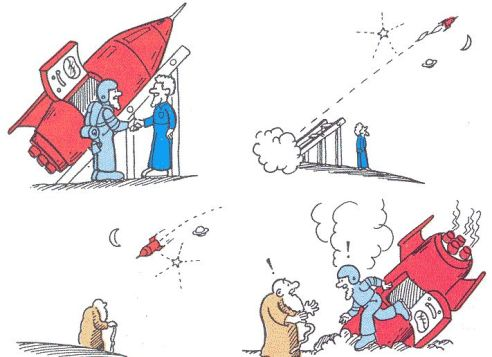
\includegraphics[width=0.65\textwidth]{img/twin_paradox.jpg}
        \end{block}
    }
\end{frame}

\begin{frame}
    \frametitle{Segundo a Física Moderna -- Relatividade Geral}
    
    \centering
    \transparent{0}\includegraphics[width=0.5\textwidth]{example-image}

    \note[item]{Do ponto de vista de um observador na origem, o deslocamento no eixo y ficou mais lento.}
    \note[item]{Do ponto de vista de um observador na origem, o tempo para o viagente passou mais lentamente.}
    \note[item]{Do ponto de vista do viajante, nada mudou.}
\end{frame}

\begin{frame}
    \frametitle{Segundo a Física Moderna -- Relatividade Geral}
    
    A gravidade é capaz de distorcer o {\em continuum} espaço-tempo.~\cite{visual-gravidade}
    
    \centering
    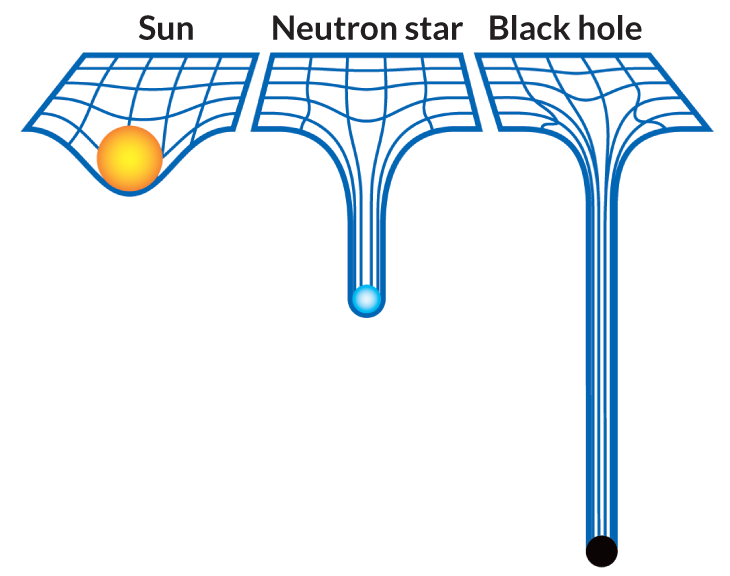
\includegraphics[width=0.6\textwidth]{img/continuum_distortion.png}

    \note[item]{O espaço-tempo foi menos esticado pelo campo gravitacional do objeto mais leve e mais pelo mais pesado.}
    \note[item]{Como se, do ponto de vista de quem ficou, quem foi fez o percurso em menos tempo.}
    \note[item]{Observável nos satélites que orbitam a terra. Necessária correção para funcionamento do GPS, por exemplo.}
\end{frame}

\begin{frame}
    \frametitle{Segundo a Física Moderna -- Relatividade Geral}
    
    \begin{block}{Viagem ao futuro é possível}
        \begin{itemize}
            \item Ponte de Einstein-Rosen. (buraco de minhoca)
        \end{itemize}
    \end{block}

    \centering
    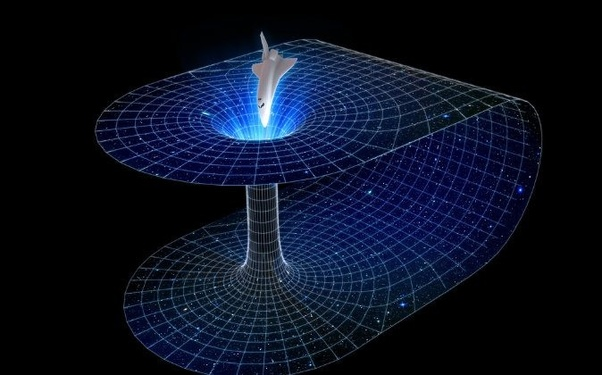
\includegraphics[height=0.6\textwidth]{img/wormhole.jpg}
    
\end{frame}

\begin{frame}
    \frametitle{Segundo a Física Moderna -- Relatividade Geral}
    
    \centering
    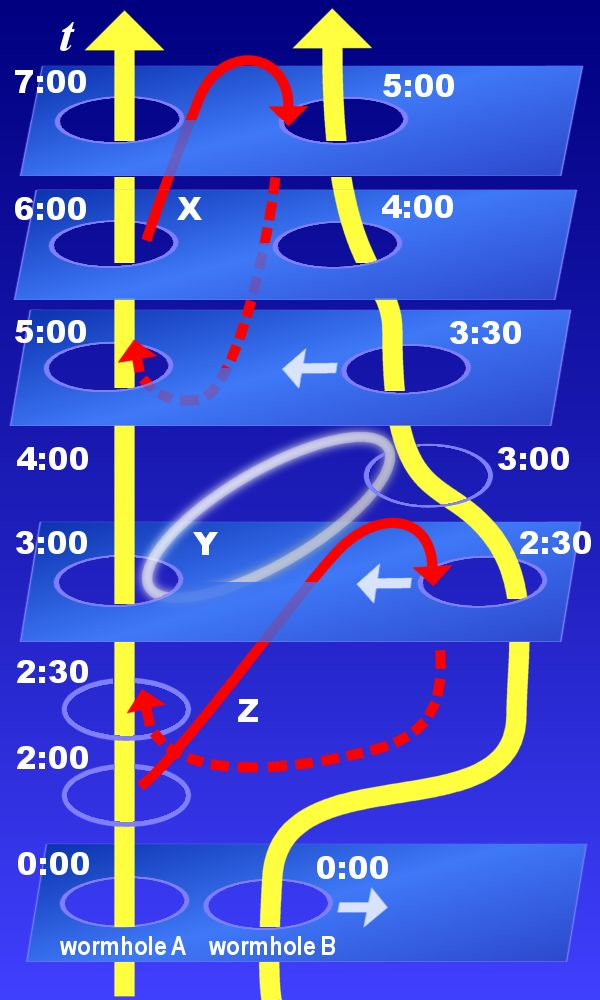
\includegraphics[height=0.75\textwidth]{img/wormhole_timetravel.jpg}
    
\end{frame}

\begin{frame}
    \frametitle{Então...}

    \alert{Dá pra viajar no tempo!} \uncover<2->{Mas dá mesmo...?}

    \begin{itemize}[<3->]
        \item Todas as soluções parecem requerer:
        \begin{itemize}
            \item Energia infinita
            \item Espaço infinito
            \item Massa negativa
        \end{itemize}
        \item<4-> E quase sempre o resultado disso termina na criação de um buraco-negro...
    \end{itemize}
\end{frame}

\subsection{Viagem ao passado}

\begin{frame}
    \frametitle{Então...}

    O problema mesmo é \alert{viajar para o passado...}
\end{frame}

\begin{frame}
    \frametitle{Paradoxos}
    
    \begin{block}{Paradoxo do Avô}
        \centering
        \transparent{0}\includegraphics[width=0.5\textwidth]{example-image}
    \end{block}

    \begin{itemize}
        \item<2-> Se eu puder voltar ao passado, para antes dos meus avós se conhecerem,
        \item<3-> encontrar e matar meu avô,
        \item<4-> eu não poderia existir.
        \item<5-> {\bfseries Mas como eu poderia ter voltado para impedi-los de se conhecer?} 
    \end{itemize}
    
    \note[item]{Contado em algumas versões, incluindo pai ou impedir sua própria viagem.}
    
\end{frame}

\begin{frame}
    \frametitle{Paradoxos}
    
    \begin{block}{Paradoxo da Predestinação}
        \centering
        \transparent{0}\includegraphics[width=0.5\textwidth]{example-image}
    \end{block}

    \begin{itemize}
        \item {\bfseries Ou será que os acontecimentos estão predestinados?}
    \end{itemize}
    
\end{frame}

\begin{frame}
    \frametitle{Paradoxos}
    
    \begin{block}{Paradoxo da Informação sem Fonte}
        \centering
        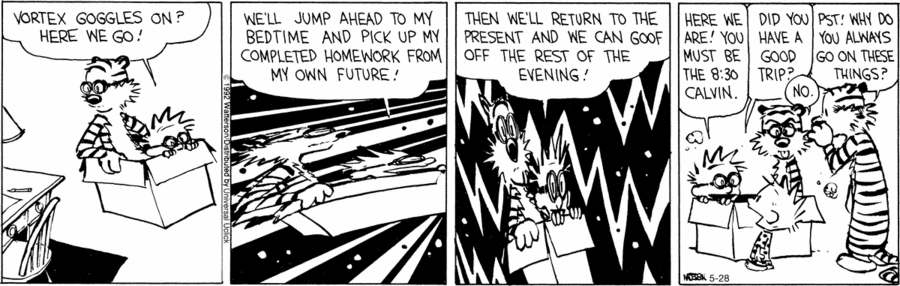
\includegraphics[width=\textwidth]{img/calvin_hobbes.png}
    \end{block}

    \begin{itemize}
        \item<2-> Se o Calvin das 8h30 possui o dever de casa feito,
        \item<3-> e o do passado puder pegar e voltar para curtir a tarde,
        \item<4-> para às 8h30 entregar o dever ao que veio do passado,
        \item<5-> {\bfseries quem fez o dever?}
    \end{itemize}
    \note[item]{Contado em algumas versões, incluindo Leonardo Da Vinci e a Mona Lisa.}
    
\end{frame}

\begin{frame}
    \frametitle{E agora?}
    
    \begin{itemize}
        \item Ao menos três teorias são possíveis:
        \begin{itemize}[<+->]
            \item Princípio da Autoconsistência de Novikov
            \item Predestinação
            \item Multiverso
        \end{itemize}
        \item<+-> Mesmo assim, ainda não se imagina como voltar para antes do momento da criação da máquina a ser usada.
        \note[item]{Frase de Stephen King: ``A viagem sendo possível, onde estão os viajantes?''}
    \end{itemize}
\end{frame}

\section{Viagem no Tempo ---  segundo a ficção (cinema)}

    \begin{frame}
    \frametitle{Spoiler Alert}

    \centering
    
    \alert{\Huge \bfseries Atenção!}
    
    {Pode conter {\em spoilers}.}
\end{frame}

\begin{frame}
    \frametitle{Ideias gerais de enredo}

    \begin{itemize}
        \item Reviver {\em , }
        \item Predestinação {\em , , Vingadores: Ultimato (queria ser)}
        \item Novos fluxos {\em , , , }
        \item Novas linhas temporais {\em Vingadores: Ultimato (na verdade é)}
        \item Consequências imediatas {\em Looper, De Volta para o Futuro}
        \item Projeção de consciência {\em X-MEN: Dias de um Futuro Esquecido, Contra o tempo}
    \end{itemize}
\end{frame}

\begin{frame}
    \frametitle{Reviver}
    
    \alert{O Feitiço do Tempo}

    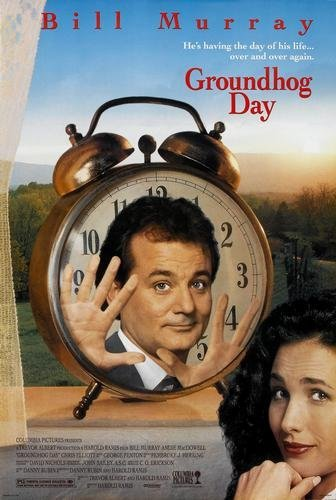
\includegraphics[height=0.8\textheight]{img/posters/groundhog_day.jpg}
\end{frame}

\begin{frame}
    \frametitle{Reviver}
    
    \alert{No Limite do Amanhã}

    
\includegraphics[height=0.8\textheight]{img/posters/edge_of_tomorrow.jpg}
\end{frame}

\begin{frame}
    \frametitle{Predestinação}
    
    \alert{Harry Potter e o Prisioneiro de Azkaban}

    
\includegraphics[height=0.8\textheight]{img/posters/hpatpoa.jpg}
\end{frame}

\begin{frame}
    \frametitle{Predestinação}
    
    \alert{Te Amarei para Sempre}

    
\includegraphics[height=0.8\textheight]{img/posters/ttw.jpeg}
\end{frame}

\begin{frame}
    \frametitle{Novos Fluxos}
    
    \alert{Questão de Tempo}

    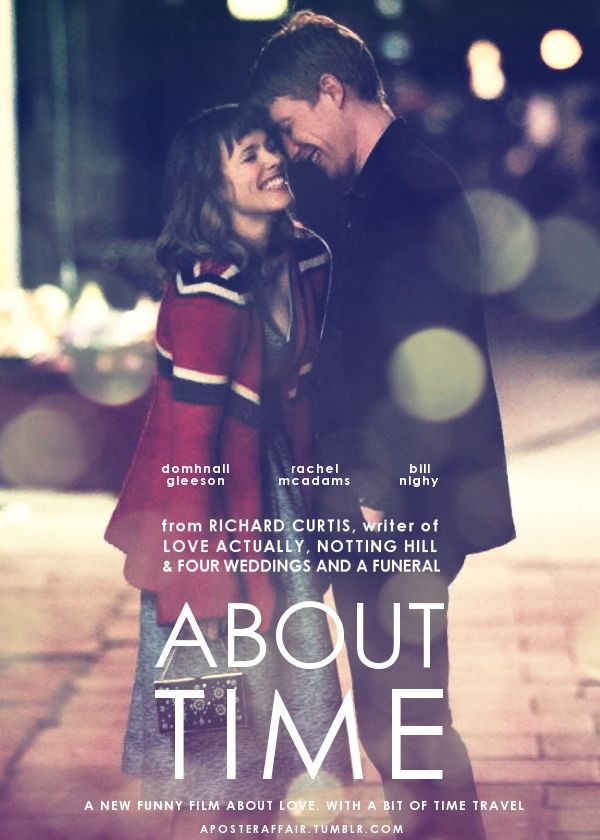
\includegraphics[height=0.8\textheight]{img/posters/about_time.jpg}
\end{frame}

\begin{frame}
    \frametitle{Novos Fluxos}
    
    \alert{Efeito Borboleta}

    
\includegraphics[height=0.8\textheight]{img/posters/butterfly_effect.jpg}
\end{frame}

\begin{frame}
    \frametitle{Novos Fluxos}
    
    \alert{Exterminador do Futuro 2 e 3}

    \begin{columns}
        \begin{column}{0.4\textwidth}
            
\includegraphics[height=0.8\textheight]{img/posters/terminator_2.jpg}
        \end{column}
        \begin{column}{0.4\textwidth}
            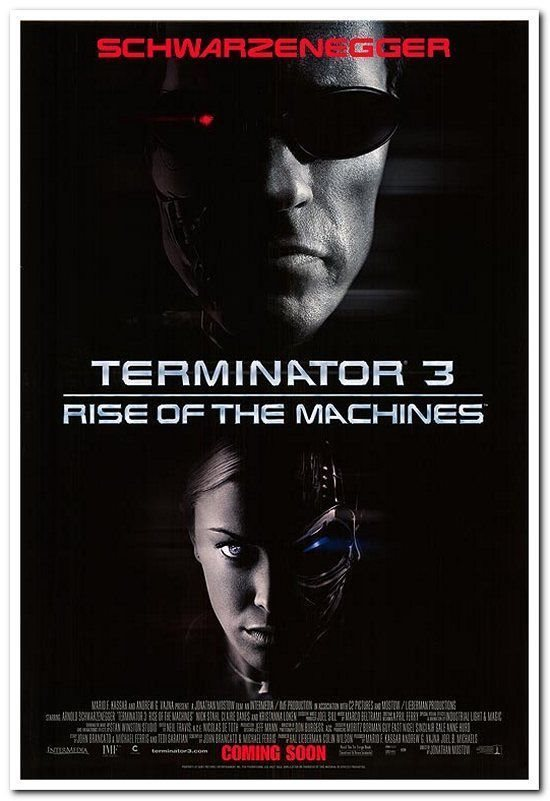
\includegraphics[height=0.8\textheight]{img/posters/terminator_3.jpg}
        \end{column}
    \end{columns}
\end{frame}

\begin{frame}
    \frametitle{Novos Fluxos}
    
    \alert{Príncipe da Pérsia}

    
\includegraphics[height=0.8\textheight]{img/posters/pop.jpg}
\end{frame}

\begin{frame}
    \frametitle{Novas Linhas Temporais}
    
    \alert{Vingadores: Ultimato}

    
\includegraphics[height=0.8\textheight]{img/posters/avengers_endgame.jpg}
\end{frame}

\begin{frame}
    \frametitle{Consequências Imediatas}
    
    \alert{Looper: assassinos do futuro}

    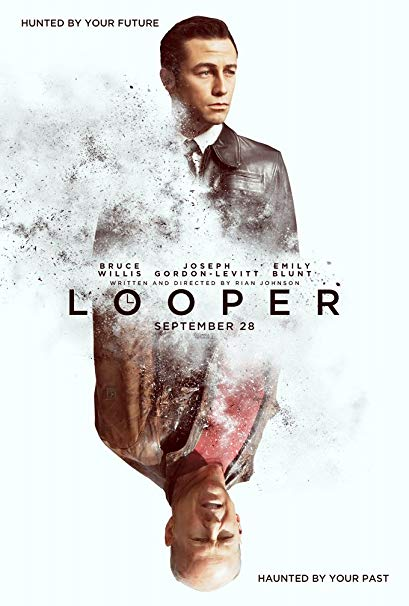
\includegraphics[height=0.8\textheight]{img/posters/looper.jpg}
\end{frame}

\begin{frame}
    \frametitle{Consequências Imediatas}
    
    \alert{De volta para o Futuro}

    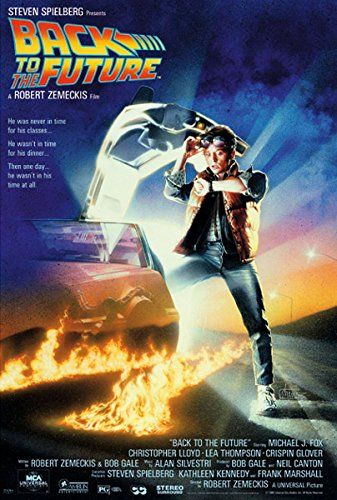
\includegraphics[height=0.8\textheight]{img/posters/bttf.jpg}
\end{frame}

\begin{frame}
    \frametitle{Projeção de Consciência}
    
    \alert{X-MEN: Dias de um Futuro Esquecido}

    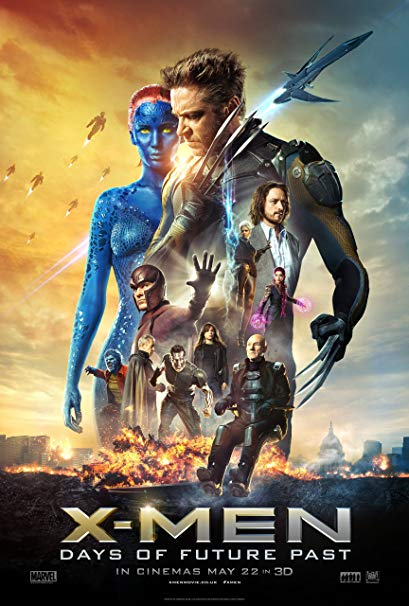
\includegraphics[height=0.8\textheight]{img/posters/xmen_dofp.jpg}
\end{frame}

\begin{frame}
    \frametitle{Projeção de Consciência}
    
    \alert{Contra o tempo}

    
\includegraphics[height=0.8\textheight]{img/posters/source_code.jpeg}
\end{frame}

\section{Estruturas de Dados Temporais}

    \begin{frame}
        \frametitle{Terminologia}

        \begin{itemize}
            \item Consultas {\em vs.} Atualizações
            \note[item]{{\em Operações:} Todas as operações que podemos realizar numa estrutura realizam alguma tarefa que pode ser classificada entre \underline{obter uma informação} (obter a resposta a uma pergunta) ou \underline{realizar uma alteração na organização}.}
            \note[item]{{\em Operações:} Existem certas operações que podem se comportar de ambas as formas, mas sempre podemos subdividí-las.}
            \item Versão
            \note[item]{{\em Versão:} Cada configuração (ou estado) de uma estrutura de dados após uma operação de Atualização.}
        \end{itemize}
    \end{frame}

    \begin{frame}
        \frametitle{Estruturas de Dados Temporais}

        \begin{itemize}
            \item Efêmeras
            \begin{itemize}[<2->]
                \item Apenas uma versão (a última) está disponível para manipulação.
                \note[item]{{\em Efêmeras:} As estruturas que chamamos de ``Estruturas de Dados''.}
                \note[item]{{\em Efêmeras:} Efêmero significa passageiro, que dura pouco. Qualquer estado da estrutura dura apenas até a próxima atualização.}
                \note[item]{{\em Efêmeras:} Modelo de memória de um computador. Uma vez feito, não se sabe o que estava lá antes.}
            \end{itemize}
            \item Persistentes
            \begin{itemize}[<3->]
                \item Todas as versões da estrutura estão disponíveis para manipulação.
                \item Atualizações em alguma versão {\em não se propagam} para as demais.
                \note[item]{{\em Persistentes:} Se comportam em analogia à visão que a física tem sobre viagem no tempo.}
            \end{itemize}
            \item Retroativas
            \begin{itemize}[<4->]
                \item Todas as versões da estrutura estão disponíveis para manipulação.
                \item Atualizações em alguma versão {\em sempre se propagam} para as demais.
                \note[item]{{\em Retroativas:} Se comportam em analogia à visão que algumas obras de ficção tem sobre viagem no tempo.}
            \end{itemize}
        \end{itemize}
    \end{frame}

    \begin{frame}
        \frametitle{Persistência {\em vs.} Retroatividade}
        
        \begin{block}{Persistência}
            \centering
            \transparent{0}\includegraphics[width=.5\textwidth]{example-image}
            \note[item]{Várias linhas do tempo. Universos paralelos.}
        \end{block}
        
        \begin{itemize}
            \item Operações ganham um novo parâmetro: {\em a versão que será o seu alvo}.
        \end{itemize}

    \end{frame}

    \begin{frame}
        \frametitle{Persistência {\em vs.} Retroatividade}
        
        \begin{block}{Retroatividade}
            \centering
            \transparent{0}\includegraphics[width=.5\textwidth]{example-image}
            \note[item]{Uma única linha do tempo.}
        \end{block}
        
        \begin{itemize}
            \item Operações ganham um novo parâmetro: {\em o ``momento'' onde serão realizadas}.
        \end{itemize}

    \end{frame}


    \begin{frame}
        \frametitle{Níveis de persistência}

        \begin{block}{Persistência parcial}
            \centering
            \transparent{0}\includegraphics[width=.5\textwidth]{example-image}
        \end{block}

        \begin{itemize}
            \item<1-> Consultas podem ser feitas sobre {\em qualquer versão}.
            \item<2-> Atualizações só podem ser feitas sobre {\em a versão mais recente}.
            \begin{itemize}
                \item<3-> Isso obriga uma distribuição totalmente ordenada das versões.
            \end{itemize}
        \end{itemize}

        \note[item]{Corresponde à forma de percepção de tempo que temos hoje. Lembramos como as coisas eram no passado, mas não podemos alterá-las.}
        \note[item]{De uma certa forma, seria como se só pudéssemos viajar ao passado para sermos ``expectadores''. Ou ainda, corresponderia às versões de ficção com fatos rígidos.}
    \end{frame}

    \begin{frame}
        \frametitle{Níveis de persistência}

        \begin{block}{Persistência total}
            \centering
            \transparent{0}\includegraphics[width=.5\textwidth]{example-image}
        \end{block}

        \begin{itemize}
            \item<1-> Consultas podem ser feitas sobre {\em qualquer versão}.
            \item<2-> Atualizações podem ser feitas sobre {\em qualquer versão}.
            \item<3-> Atualizações não afetam versões já existentes, o que obriga uma ``ramificação'' entre as versões.
            \begin{itemize}
                \item<4-> Isso obriga uma distribuição das versões como uma árvore.
            \end{itemize}
        \end{itemize}

        \note[item]{Corresponde à forma de viagem no tempo de ``universos paralelos''.}
    \end{frame}

    \begin{frame}
        \frametitle{Níveis de persistência}

        \begin{block}{Persistência confluente}
            \centering
            \transparent{0}\includegraphics[width=.5\textwidth]{example-image}
        \end{block}

        \begin{itemize}
            \item Persistência total +
            \item<2-> É possível ``mesclar'' duas ou mais versões em uma nova versão.
        \end{itemize}

        \note[item]{Difícil de imaginar um correspondente quanto a viagem no tempo.}
        \note[item]{Parece haver uma série de televisão antiga que faz uso desse conceito: {\em Sliders}.}
        \note[item]{Corresponde à forma como funcionam os sistemas de controle de versão.}
    \end{frame}

    \begin{frame}
        \frametitle{Níveis de persistência}

        \begin{block}{Persistência funcional}
            \centering
            \transparent{0}\includegraphics[width=.5\textwidth]{example-image}
        \end{block}

        \begin{itemize}
            \item \underline{Nada} pode ser alterado. Toda modificação deve preservar a memória anterior intacta.
        \end{itemize}

        \note[item]{Difícil de imaginar um correspondente quanto a viagem no tempo.}
        \note[item]{Se inspira na forma de comportamento de linguagens funcionais.}
        \note[item]{Se diferencia das demais, pois anteriormente poderíamos alterar parte da memória, desde que o acesso e a interpretação das versões anteriores fosse preservado.}
        \note[item]{Inclui a capacidade de todas as anteriores, já que como nada é alterado, nada é perdido.}
    \end{frame}

    \begin{frame}
        \frametitle{Níveis de retroatividade}

        \begin{block}{Retroatividade parcial}
            \centering
            \transparent{0}\includegraphics[width=.5\textwidth]{example-image}
        \end{block}

        \begin{itemize}
            \item<1-> Atualizações podem ser adicionadas ou removidas em qualquer ``momento'' no passado.
            \item<4-> Consultas só podem ter como alvo o ``momento presente''.
        \end{itemize}

        \note[item]{Seria como mandar alguém para o passado e manter a consciência de como o presente se altera.}
        \note[item]{A física moderna não permite conceber esse tipo de viagem no tempo.}
        \note[item]{Podem acontecer ``paradoxos''.}
        \note[item]{MIB 3}
    \end{frame}

    \begin{frame}
        \frametitle{Níveis de retroatividade}

        \begin{block}{Retroatividade total}
            \centering
            \transparent{0}\includegraphics[width=.5\textwidth]{example-image}
        \end{block}

        \begin{itemize}
            \item<1-> Atualizações podem ser adicionadas ou removidas em qualquer ``momento'' no passado.
            \item<2-> Consultas podem ser adicionadas ou removidas em qualquer ``momento'' no passado.
            \begin{itemize}
                \item<3-> Alterações têm um impacto muito maior (reação em cadeia).
            \end{itemize}
        \end{itemize}

        \note[item]{Seria como você ir para o passado e interferir com o andamento dos acontecimentos.}
        \note[item]{Podem acontecer ``paradoxos''.}
    \end{frame}

    \begin{frame}
    \frametitle{Existem? São úteis?}

    \begin{itemize}
        \item Funcionamento do Git
        \item Frameworks como React
        \item Modelo de memória de linguagens funcionais
        \item Modelo de execução para alguns MMOGs.
        \item Auxiliares na resolução de alguns problemas
        \note[item]{Economizam espaço, facilitam raciocínio sobre fluxo de dados, abreviam tempo de resposta}
    \end{itemize}
\end{frame}

    \begin{frame}
    \frametitle{Tornando persistente}

    \begin{itemize}
        \item Forma mais trivial: guardar tudo!
        \item Forma mais inteligente: reaproveitar memória.
    \end{itemize}

    \begin{itemize}
        \item No modelo de Máquina de Ponteiros, somos capazes de:
        \begin{itemize}
            \item Parcialmente persistente: $O(n)$, $O(\lg n)$
            \item Totalmente persistente: $O(m)$, para alguns casos
            \item Confluente, Funcional, Retroativo: {\em quase tudo está em aberto}
        \end{itemize}
    \end{itemize}
\end{frame}

\section{Um último enredo a analisar}

    {
    \usebackgroundtemplate{\transparent{0.4}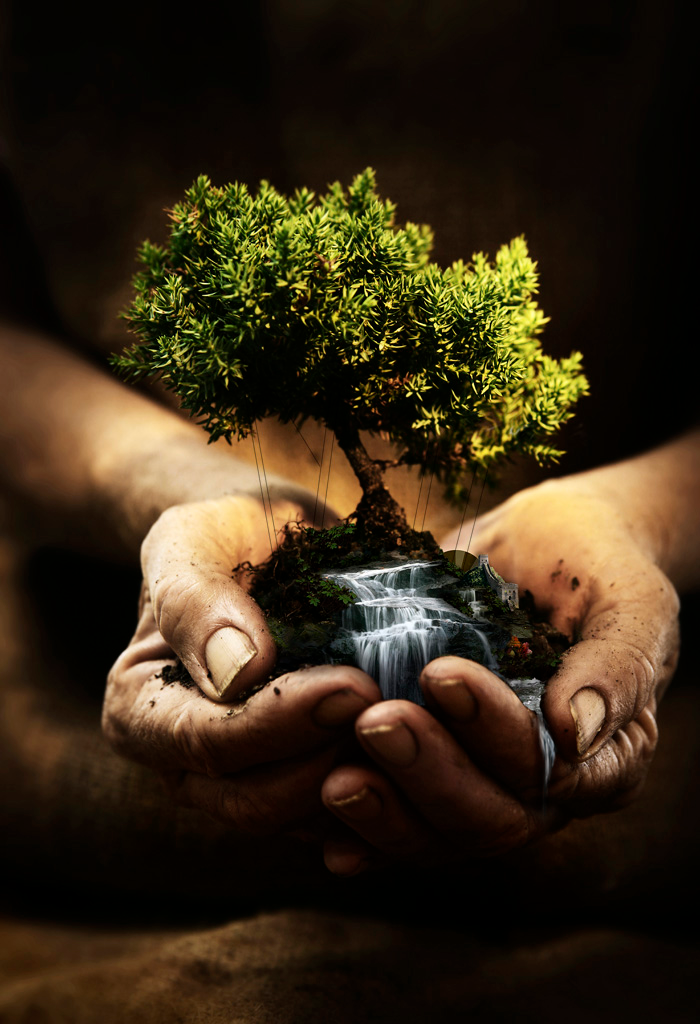
\includegraphics[height=\paperheight]{img/save_the_nature.png}}
    \begin{frame}

        \setbeamercolor{item}{fg=black}
        \setbeamercolor{normal text}{fg=black}
        \usebeamercolor[fg]{normal text}
        \begin{aquote}{???~\cite{abcd}}
            Imagine um mundo onde viagem no tempo não exista, nem seja possível. \pause Onde suas ações são imutáveis e você só tenha uma chance. \pause E onde não existam reviravoltas para salvar o dia no final. \pause {\bfseries O que você faria?}
        \end{aquote}
    \end{frame}
    }

    \begin{frame}[allowframebreaks]
        \frametitle{Referências}

        \begin{thebibliography}{99}
            \bibitem{abcd} De: {\bfseries A take on time travel paradoxes} (em tradução livre). Disponível em \url{https://youtu.be/SZMFPR2Xr0Q}.
            \bibitem{visual-gravidade} {\bf Gravity Visualized}. Disponível em \url{https://youtu.be/MTY1Kje0yLg}
        \end{thebibliography}
    \end{frame}
\end{document}